\section{Comparison with experimental data}
Experimental setups have a few limitations compared to the theoretical treatment, for example you do not have complete freedom of changing the resistance, rather the resistance is changed by changing the temperature of the sample.
This has a few consequences: 
\begin{itemize}
    \item Since out sample is a semiconductor, the lower the temperature, the higher the resistance, but if the temperature gets too low we enter the ballistic regime, and our treatment is no longer valid.
    \item If the temperature gets too high, the quantization of the hall effect disappears
\end{itemize}
This restricts us to a couple order of magnitude of the resistivity.

Now we compare the results with the experimental data. Let's start from analyzing the data from  \cite{rebecca2022moirè}.\\
In this paper the authors measured the valley hall effect of a heterostructure made of bilayer-graphene on top of boron nitride at different angles $\phi$ between the graphene and the boron nitride. The sample has a width $W=1.7\mu$m, and inter-valley scattering length $l_{\textrm v}=1.6\mu$m and the distance of the contact from the injection point is $x=2.3\mu$m

The angles $\phi$ that were explored are $0,\pi/6$ and $\pi/3$. If you plot the measurements you get figure \ref{fig:rebeccadatapoints}.\\
\begin{figure}[h!]
    \centering
    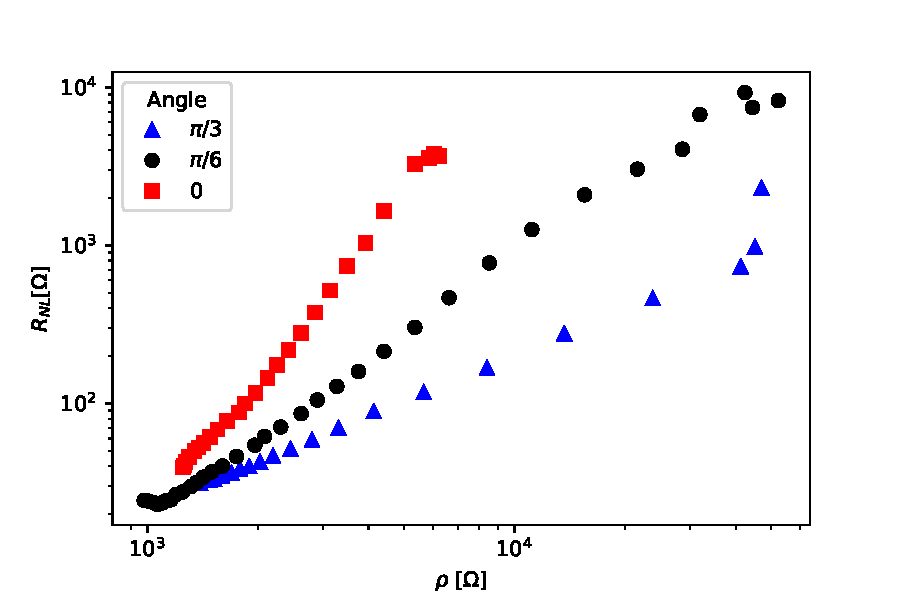
\includegraphics[width=\linewidth]{Immagini/rnl/rebecca_data.pdf}
    \caption{Datapoints from \cite{rebecca2022moirè}}
    \label{fig:rebeccadatapoints}
\end{figure}
We then analyze the data by comparing the output of the model thus far developed to the data, we did not fit the data, rather we used the knowledge we already have about the parameters $W,l_\textrm{v},x$ and plot the result on top of the datapoints.
\begin{itemize}
    \item For $\phi=\pi/3$ we have that the response is fully ohmic, and so we get a completely linear response (figure \ref{fig:rebecca pi/3})
    \item For $\phi=\pi/6$ we have a hall effect, however, since $W\approx l_\textrm{v}$ the ohmic and the topological response mix together, so we never see the full-fledged $\rho^3$ behavior.\footnote{A more detailed explanation was given in the details of subsection \ref{sec:alternaterho}}
    \item For $\phi=0$ the response does not match the model we developed, further investigations should be done to address the discrepancy
\end{itemize}
\begin{figure}[h!]
    \centering
    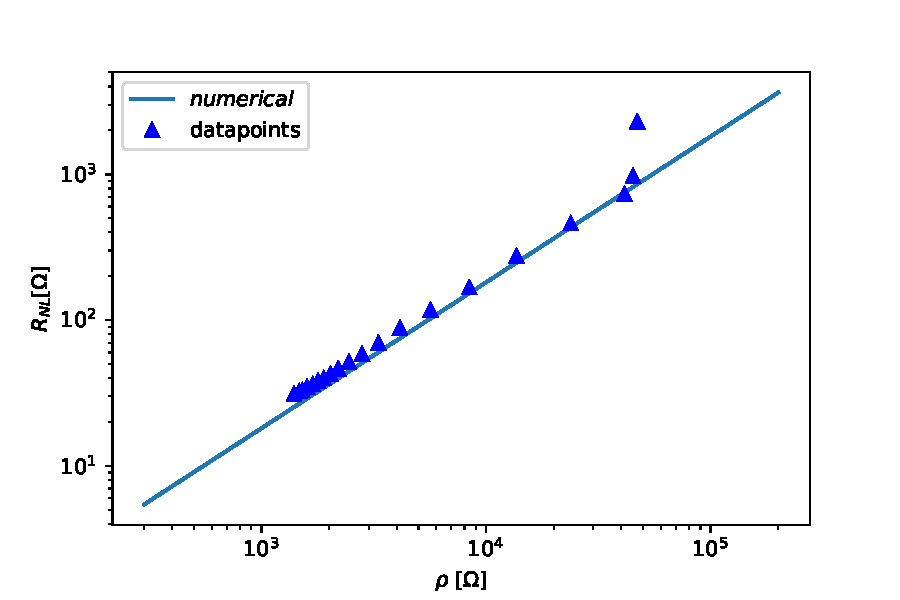
\includegraphics[width=\linewidth]{Immagini/rnl/rebecca_0.pdf}
    \caption{Comparison between the data points and the theoretical expectation for $\phi=\pi/3$. With the exception of the last experimental point, the data follows the theoretical prediction}
    \label{fig:rebecca pi/3}
\end{figure}
\begin{figure}[h!]
    \centering
    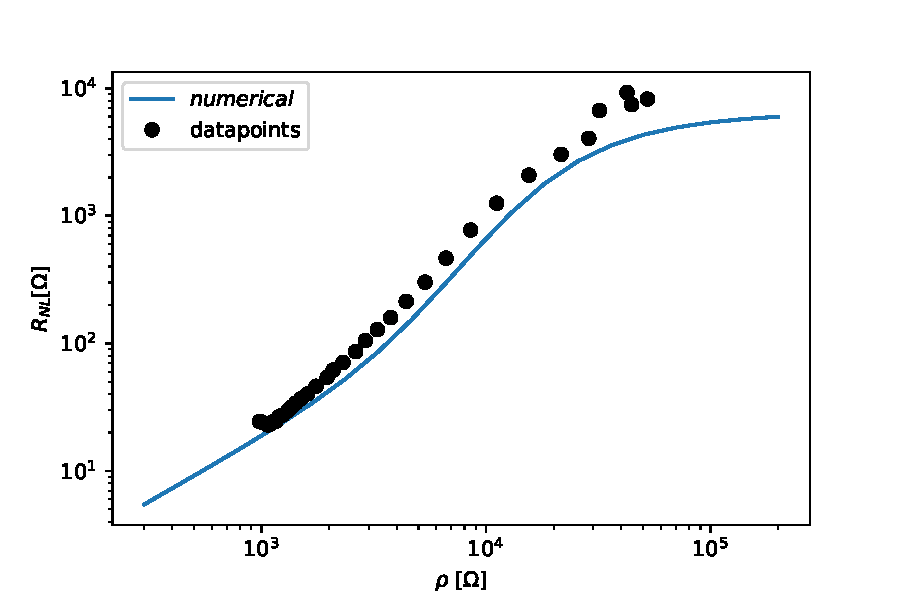
\includegraphics[width=\linewidth]{Immagini/rnl/rebecca_1.pdf}
    \caption{Comparison between the data points and the theoretical expectation for $\phi=\pi/6$. The model has a lower precision for higher values of $\rho,R_{\textrm{NL}}$, however we can say that the data follow the theoretical prediction}
    \label{fig:rebecca pi/6}
\end{figure}
\begin{figure}[h!]
    \centering
    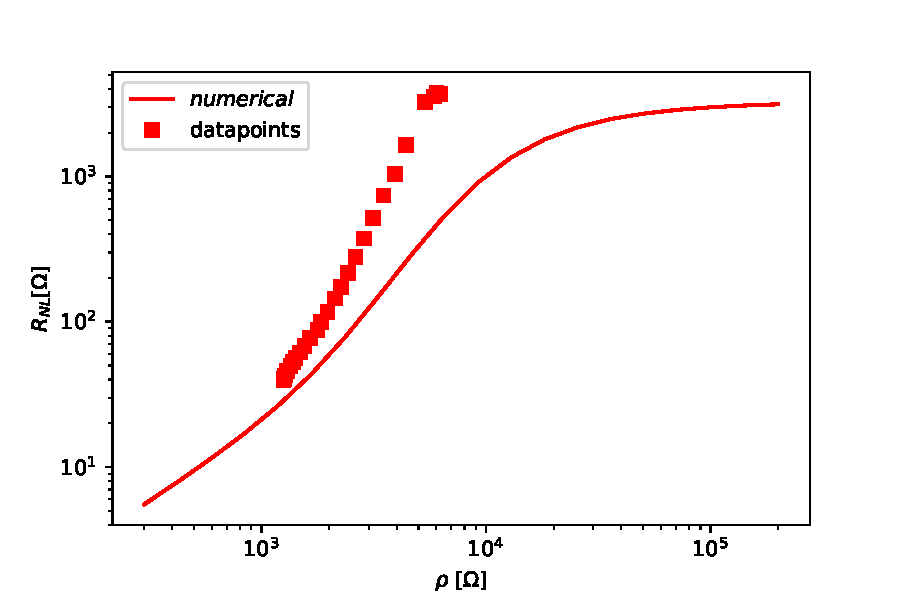
\includegraphics[width=\linewidth]{Immagini/rnl/rebecca_2.pdf}
    \caption{Comparison between the data points and the theoretical expectation for $\phi=0$. The model does not satisfactorily reflect the data.}
    \label{fig:rebecca 0}
\end{figure}

\section{Conclusions}
In this thesis we provided a complete and accurate description on the Nonlocal resistance arising from valley-Hall. It expands on top of the work done by Beconcini et al. \cite{Beconcini_2016} where they manage to explain the results Shimazaki et al. obtained  \cite{shimazaki2015generation} where they found a that the non-linear resistance on bilayer graphene depended on the cube of the longitudinal resistivity ($R_\textrm{NL}\propto \rho^3$) for low resistivities and then it saturates.\\ 
The work done by Beconcini et al. was only able to explain the behavior of the nonlocal resistance if the width of the material is much smaller than the valley diffusion length ($l_v\ll W$). In this thesis we found an accurate description for any valley diffusion length and width and we compared the results with the work done by Arrighi et al. \cite{rebecca2022moirè}.
The results we obtained can also be used to study the non-local resistance of other anomalous Hall effect such as spin-Hall effect.